% !TEX program = xelatex
% Generated by slide-forge + Claude
\documentclass[aspectratio=169]{beamer}
\usepackage[utf8]{inputenc}
\usepackage{amsmath,amssymb}
\usepackage{booktabs}
\usepackage{graphicx}
\usepackage{pifont}
\graphicspath{{figures/}}

\usetheme{Perelyn}

\title{Graph-Structured Memory for Cognitive Agents}
\subtitle{From Knowledge Graphs to Non-Euclidean Geometry}
\author{Michael Banf}
\institute{Perelyn GmbH, Munich}
\date{FGWM @ KI 2026}

\begin{document}

\begin{frame}[plain]
  \titlepage
\end{frame}

\begin{frame}{Overview}
  \tableofcontents
\end{frame}

%% ==========================================================================
%% SECTION 1 — Why Graph Memory?
%% ==========================================================================
\section{Why Graph Memory?}

\begin{frame}[plain]
  \sectionpage
\end{frame}

\begin{frame}{The Limits of Flat Memory}
  \begin{itemize}
    \item LLM agents need memory that \alert{spans sessions}, tracks change,
      and supports multi-hop reasoning
    \item Dominant approaches: vector stores, key-value extraction, or
      brute-force context compression
    \item These work for factual recall --- but fail systematically on:
    \begin{itemize}
      \item \alert{Temporal reasoning} --- what changed and when?
      \item \alert{Multi-hop inference} --- connecting facts across steps
      \item \alert{Knowledge evolution} --- updating beliefs over time
    \end{itemize}
  \end{itemize}

  \vspace{0.3cm}

  \begin{block}{Benchmark Evidence}
    Cognitive accuracy below 25\% across Mem0, Letta, and Zep (LoCoMo-Plus, 2026).\\
    Multi-hop conflict resolution below 7\% for all methods (MemoryAgentBench).
  \end{block}
\end{frame}

\begin{frame}{Graph Memory: A Different Strategy}
  \begin{columns}[T]
    \begin{column}{0.48\textwidth}
      \textbf{Instead of compressing everything:}
      \begin{itemize}
        \item Store knowledge in a \alert{graph}
        \item Retrieve \alert{selectively} via topology
        \item Entities and relations are first-class
        \item Temporal intervals on edges
      \end{itemize}

      \vspace{0.3cm}

      {\small Multi-strategy graph systems achieve 91.4\% retrieval
      vs.\ 49.0\% for extraction-based (LongMemEval).}
    \end{column}

    \begin{column}{0.48\textwidth}
      \centering
      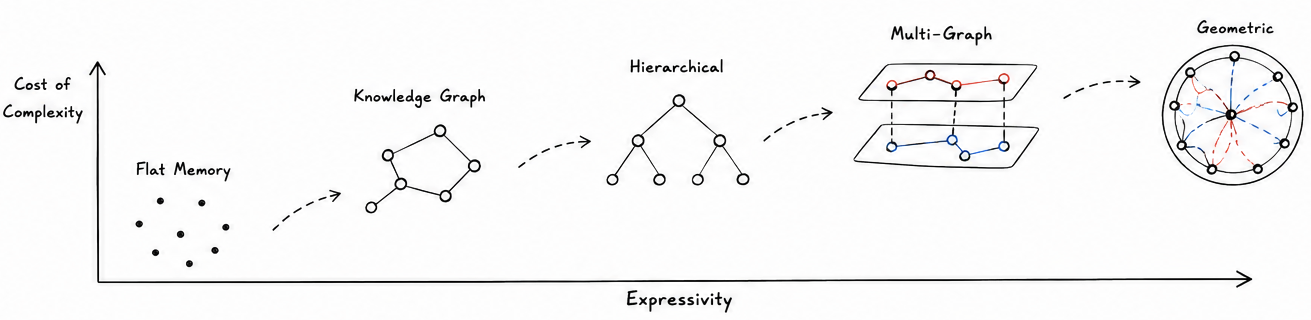
\includegraphics[width=\textwidth]{overview.png}

      \vspace{0.2cm}

      {\footnotesize Progression from flat memory to geometric representations.}
    \end{column}
  \end{columns}
\end{frame}

%% ==========================================================================
%% SECTION 2 — Taxonomy
%% ==========================================================================
\section{Graph Memory Taxonomy}

\begin{frame}[plain]
  \sectionpage
\end{frame}

\begin{frame}{Six Architectural Patterns}
  \begin{columns}[T]
    \begin{column}{0.48\textwidth}
      \textbf{Established:}
      \begin{enumerate}
        \item \alert{Entity-relation KGs} --- typed triples\\
          {\small (GraphRAG, CraniMem, AriGraph)}
        \item \alert{Hierarchical event graphs} --- episodic + semantic layers\\
          {\small (GAM, MemFly, MemGraphRAG)}
        \item \alert{Bipartite / associative} --- lightweight linking\\
          {\small (LP-RAG, AssoMem)}
        \item \alert{Multi-graph composites} --- orthogonal views\\
          {\small (MAGMA, TM2RAG)}
      \end{enumerate}
    \end{column}

    \begin{column}{0.48\textwidth}
      \textbf{Emerging:}
      \begin{enumerate}
        \setcounter{enumi}{4}
        \item \alert{Hypergraph memory} --- $n$-ary facts\\
          {\small (HyperGraphRAG, HyperMem)}
        \item \alert{Procedural strategy graphs} --- agent trajectories\\
          {\small (TGM, PRAXIS, SkillRL)}
      \end{enumerate}

      \vspace{0.4cm}

      \begin{block}{Key Finding}
        Entity-relation KGs account for \alert{60\%} of surveyed systems.
        Non-KG structures remain rare.
      \end{block}
    \end{column}
  \end{columns}
\end{frame}

\begin{frame}{The Temporal Grounding Deficit}
  \begin{itemize}
    \item Despite being the central promise, \alert{57\%} of surveyed systems
      implement \alert{no temporal mechanism}
    \item Only 20\% go beyond simple timestamps
    \item Best solution: Graphiti/Zep with \alert{bi-temporal model}\\
      {\small (event time vs.\ ingestion time, validity intervals on every edge)}
  \end{itemize}

  \vspace{0.3cm}

  \begin{columns}[T]
    \begin{column}{0.48\textwidth}
      \textbf{What exists:}
      \begin{itemize}
        \item RecallM --- temporal windows
        \item MemoTime --- time trees
        \item Mnemosyne --- exponential decay
      \end{itemize}
    \end{column}
    \begin{column}{0.48\textwidth}
      \textbf{What's missing:}
      \begin{itemize}
        \item \alert{Staleness tracking} for semantic knowledge
        \item Continuous-time evolution
        \item Principled temporal fusion
      \end{itemize}
    \end{column}
  \end{columns}
\end{frame}

%% ==========================================================================
%% SECTION 3 — Retrieval
%% ==========================================================================
\section{Retrieval Spectrum}

\begin{frame}[plain]
  \sectionpage
\end{frame}

\begin{frame}{From Graph Algorithms to Learned Retrieval}
  \begin{itemize}
    \item \textbf{Training-free} (dominant): PageRank, Leiden, recency decay
      --- 10--150\,ms, works on any graph
    \item \textbf{Multi-strategy}: semantic + BM25 + graph traversal +
      temporal, fused via cross-encoder {\small (91.4\% on LongMemEval)}
    \item \textbf{RL-based}: learned edge weights, memory operations,
      graph construction
    \item \textbf{GNN message passing}: only a handful of systems
      {\small (cold start and evolution barriers)}
  \end{itemize}

  \begin{alertblock}{The Model-Size Equalizer}
    Graph memory disproportionately benefits smaller models.
    GAM: +39\% F1 at 7B, only +7\% at GPT-4o.
    Trained 4B with graph memory outperforms baseline 8B.
  \end{alertblock}
\end{frame}

%% ==========================================================================
%% SECTION 4 — Geometric Frontier
%% ==========================================================================
\section{The Geometric Frontier}

\begin{frame}[plain]
  \sectionpage
\end{frame}

\begin{frame}{Why Geometry Matters}
  \begin{columns}[T]
    \begin{column}{0.48\textwidth}
      \textbf{The problem:}
      \begin{itemize}
        \item All surveyed systems embed graphs in \alert{flat Euclidean space}
        \item But memory graphs are inherently \alert{hierarchical} and tree-like
        \item Euclidean volume grows polynomially ---\\
          tree branching grows \alert{exponentially}
        \item Result: \alert{semantic collapse} as memory grows
      \end{itemize}
    \end{column}

    \begin{column}{0.48\textwidth}
      \textbf{The intuition:}
      \begin{itemize}
        \item \alert{Hyperbolic space} has exponential volume growth
          --- naturally separates hierarchy levels
        \item Abstract topics near the center,\\
          specific facts near the boundary
        \item \alert{Curvature diagnostics} flag retrieval bottlenecks
          without training
        \item Already proven in knowledge graph reasoning
      \end{itemize}
    \end{column}
  \end{columns}

  \vspace{0.3cm}

  {\small Recent evidence: LLM token embeddings already exhibit negative Ricci curvature ---
  suggesting LLM representations are naturally hyperbolic (HELM, 2025).}
\end{frame}

\begin{frame}{Three Geometric Techniques}
  \begin{enumerate}
    \item \textbf{Discrete Ricci curvature} --- per-edge diagnostic\\
      {\small Flags bottleneck edges causing over-squashing.
      Training-free, $O(|E|)$.}

    \vspace{0.2cm}

    \item \textbf{Hyperbolic embeddings} --- hierarchy-preserving retrieval\\
      {\small Drop-in replacement for Euclidean representations.
      HyperbolicRAG, HypRAG show gains.}

    \vspace{0.2cm}

    \item \textbf{Lie group manifolds} --- temporal knowledge fusion\\
      {\small Entities, relations, timestamps in different spaces ---
      Lie algebra enables principled fusion.}
  \end{enumerate}

  \vspace{0.1cm}

  {\small Plus: mixed-curvature product spaces for heterogeneous graphs (GraphMoRE).}
\end{frame}

\begin{frame}{Concrete Example: Enhancing Graphiti/Zep}
  \begin{block}{Starting point: strongest bi-temporal system in our survey}
    Entity-relation KG with validity intervals on every edge.
  \end{block}

  \vspace{0.2cm}

  \begin{enumerate}
    \item \textbf{Curvature diagnostic} --- Forman-Ricci curvature
      \alert{flags retrieval bottlenecks} automatically\\
      {\small No training needed. Explains the cognitive accuracy ceiling.}

    \vspace{0.1cm}

    \item \textbf{Hyperbolic embeddings} --- Poincar\'{e} ball replaces
      Euclidean entity vectors\\
      {\small Abstract topics near center, specific facts near boundary.}

    \vspace{0.1cm}

    \item \textbf{Temporal fusion} --- $SO(2)$ rotations fuse validity
      intervals with embeddings\\
      {\small Answer \emph{what}, \emph{when}, and \emph{how beliefs evolved}.}
  \end{enumerate}

  \vspace{0.1cm}

  \alert{None require retraining the LLM} --- they operate on the memory layer.
\end{frame}

%% ==========================================================================
%% SECTION 5 — Takeaway
%% ==========================================================================
\section{Takeaway}

\begin{frame}[plain]
  \sectionpage
\end{frame}

\begin{frame}{Key Takeaway}
  \begin{block}{The Central Argument}
    The structural limitations of graph-based agent memory are consequences of a
    \alert{geometric mismatch}. Non-Euclidean techniques directly address them.
  \end{block}

  \vspace{0.2cm}

  \begin{itemize}
    \item Graph memory \alert{works} --- top benchmark scores,
      disproportionate gains for smaller models
    \item \alert{Temporal grounding deficit} (57\% of systems) is the most urgent gap
    \item Geometric techniques \alert{proven in adjacent fields} ---
      several are training-free
    \item \textbf{Open challenge:} integrating into persistent,
      cross-session architectures
  \end{itemize}

  \vspace{0.2cm}

  {\footnotesize Banf, Kuhn, Garcarz, Imasheva, Filipiak, Stiller, Mader, Kalek,
  Schattauer, Steuer, Luczyna, G\"artner, Rasenecker, Becker, Fetz --- Perelyn GmbH}
\end{frame}

%% ==========================================================================
%% DISCUSSION
%% ==========================================================================

\begin{frame}{Discussion}
  \centering
  \vfill
  {\Large\bfseries Questions \& Discussion}
  \vfill

  \begin{itemize}
    \item How does your system handle memory that evolves over time?
    \item Which structural limitation --- multi-hop ceilings, temporal gaps,
      or semantic collapse --- resonates most with your experience?
    \item Should geometric representations be built into the memory layer
      or remain a post-processing step?
  \end{itemize}
  \vfill

  {\small michael.banf@perelyn.com}
\end{frame}

%% ==========================================================================
%% CLOSING
%% ==========================================================================
\begin{frame}[plain]
  \titlepage
\end{frame}

\end{document}
